
\documentclass{../download/tPRS2e}

\usepackage{graphicx}
\graphicspath{{media/}}

\begin{document}

\title{Some Optimization Models of Tool Path Problem for Sheet Cutting Machines}

\author{
\name{
Petunin A.A.\textsuperscript{a},
Chentsov P.A.\textsuperscript{b}\textsuperscript{a},
Polishuk E.G.\textsuperscript{a},
Ukolov S.S.\textsuperscript{a}$^{\ast}$\thanks{$^\ast$Corresponding author. Email: s.s.ukolov@urfu.ru}
}
\affil{\textsuperscript{a}Ural Federal University, Yekaterinburg, Russia;
\textsuperscript{b}Institute of Mathematics and Mechanics, Ural Branch of the Russian Academy of Sciences, Yekaterinburg, Russia}
}

\maketitle

\begin{abstract}
TODO
\end{abstract}

\begin{keywords}
    thermal cutting;
    discrete optimization;
    toolpath routing;
    technological constraints;
    dynamic programming;
    thermal deformations
\end{keywords}

The problem of cutting tool path optimization
is one of the applied optimization problems arising
in the design of control programs for CNC plate cutting machines.
The cost or time spent is typically used
as objective function to optimize.
The control program is generated by special software 
(Computer-Aided Manufacturing, CAM-system)
just after another well-known optimization problem
has been solved,
i.e. the problem of nesting
(optimal placement of parts to manufacture on the plate).
The task is to minimize the consumption of sheet material
to produce the parts of known shapes, sizes and quantity.
The example of nesting of 24 parts bounded by 30 closed contours
in rectangular area with minimal distance specified is at Fig. \ref{nezting}.
This nesting was obtained by means of Integrated CAD / CAM ``Sirius''.

\begin{figure}[h]
    \begin{center}
    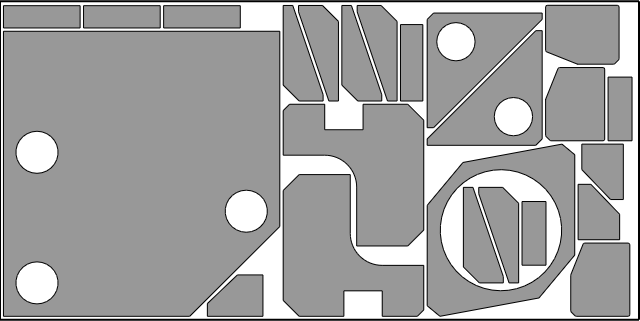
\includegraphics{nesting.png}
    \caption{Example of nesting to a sheet of $2000 \times 1000$ mm
    with minimal distance of $10$ mm}
    \label{nezting}
    \end{center}
\end{figure}

XXX \ref{nezting}.

\section{Introduction}

\section*{Acknowledgements}

The work was supported by Act 211 Government of the Russian Federation, contract № 02.A03.21.0006

\bibliographystyle{../download/tPRS}
\nocite{*}
\bibliography{en}

\end{document}
